%!TEX root = ../thesis.tex

\chapter{Approach}
\label{ch:approach}

The general approach taken to fulfill the project's goals can be summarized as follows.

To subdivide assignments into tasks, teachers will create and push markdown files to \textit{tests}.
Each task has a title and body, which is described by the contents of one of these files.
For every task a teacher creates, QuickFeed creates a GitHub issue on all student repositories in a course to represent them.
These issues have the same title and body as the task they are based on.
This way, issues are used as a representation of tasks accessible to students.

To solve a task, students will create a pull request for the issue that represents that task.
When students push code to pull requests, QuickFeed will run tests on it, similarly to the way it currently tests entire assignments.
Based on the results from a given test run, QuickFeed publishes feedback on the relevant pull request.
Furthermore, when enough tests pass, we assign one teacher and co-student to review the pull request.
Only when the teacher approves the pull request, can it be merged.

This general approach can be visualized in Figure \ref{fig:approach}.
It shows a single task that serves as the basis for individual issues on three different student repositories.
For each of these issues, a pull request is created to solve the task the issue is based on.

\begin{figure}[ht]
    \centering
    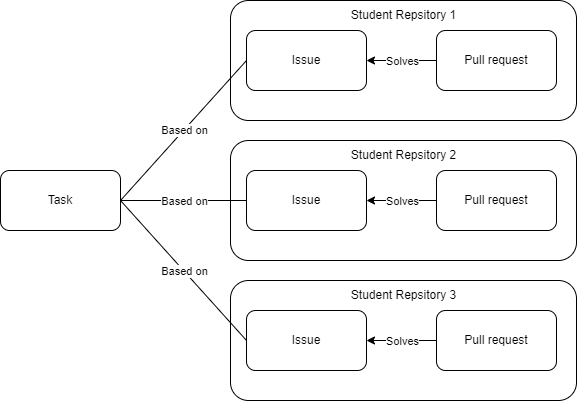
\includegraphics[scale=0.5]{photos/approach.png}
    \caption{General approach}
    \label{fig:approach}
\end{figure}

Before we can implementing anything, there are a few lingering design decisions regarding this approach.
For instance, how do we publish automatic feedback to a pull request?
In this chapter we discuss and analyse these design decisions, and try to give a rationale for the decisions that were made.

\section{Student Repository Access}
\label{sec:student-repositoriy-access}

Since students do not have access to other students' repositories, they have no easy way of accessing their code.
This becomes a necessity when doing co-student code review, as they must somehow be given access to the relevant pull request.
In this section we discuss possible solutions to overcome this problem.

\subsection{Possible Solutions}

A solution could be to use GitHub teams, a feature that would allow us to grant limited access to individual repositories.
When a student is assigned to review someone else's pull request, such a team can be created with read rights to the relevant repository.
Once the review is finished, we can either remove the team from the repository, remove the student from the team, or just delete the team altogether.
This solution does however have some unwanted side effects, which can be illustrated with the following scenario.

Imagine we have two students: A and B.
Student A is finished with a task from assignment 1, and therefore gets a reviewer assigned.
Student B is assigned to review it, and is granted access by QuickFeed to student A's repository.
Student A is also diligent, and has already started working on assignment 2.
In fact, student A has nearly completed assignment 2.
Student B however, has not even started on assignment 2, but because they can now access student A's assignments, they see how he/she did it.

As a consequence, using GitHub teams would mean that assignments can only be published after the deadline of the previous one is passed.
A prospect that would probably not be appealing to most teachers.

Another possible solution is to create a clone repository, containing only the relevant assignment. 
This way, any reviewing student will only have access to the assignment in question.
QuickFeed would create these repositories when needed, and then delete them once the review is complete.

Implementing this however seems highly complex, as there is a myriad of complications and problems that will have to be accounted for.
For one, QuickFeed must be expanded to handle, amongst other things, the following.

\begin{itemize}
    \item Creating clone repositories containing only the assignment that is relevant, and the accompanying pull request.
    \item Deleting these repositories when they are no longer needed.
    \item Associating actions on the original repository with the new one.
    I.e., we must make sure that any relevant additions to the original repository are reflected in the cloned one.
    \item Account for all possible complications that may occur.
\end{itemize}

An implementation like this also assumes that only one review is required per assignment, when there could in fact be several.
If for example an assignment has three tasks, and therefore three related pull requests, how do we then create these clone repositories?
Would we create one per pull request?
This seems like a terrible approach, as the number of repositories created would become enormous in courses with many students.

Let us say that we, despite these challenges, managed to create a fully functional implementation of the above solution.
We now have to cope with the prospect of having further complexified the user experience.
Possibly so much so that the entire solution might be counter-productive.

\subsection{Limiting Scope to Group Repositories}

The two solutions proposed in the previous section either seem too complex, or somewhat suboptimal.
Instead of going through with one of them, a compromise was agreed on to limit the project scope to only group assignments.
This means that instead of students reviewing each other's code on regular assignments, they will only do so on group assignments.
Furthermore, students will also only review other group members' pull requests.

As an example, we can imagine a group assignment with three different tasks.
A group of three students would then create one pull request each, with every member solving one task.
They are then each assigned, when appropriate, to review one of the other group members' pull request.

The benefit of this approach is that it avoids students needing access to other repositories all together.
We only need to manage student review within a local group scope, and not for an entire course.

One disadvantage is that teachers will have to more carefully plan out the tasks they create.
Say we have a group of four members, and an assignment with only three tasks.
One of the tasks will then have to be shared by two of the group members.
If every task is equally challenging to solve, it would put the other two members at a disadvantage.
It seems then that teachers should only create as many tasks as there are designated group members, or at least a multiple of that number.

Another consideration teachers will have to account for, is that they have to create tasks that are independent of each other.
If task A is dependent on task B being complete, a consequence would be group members potentially having to wait for each other.

\section{Creating Pull Requests}
\label{sec:creating-pull-requests}

Having limited our approach to only group assignments in the previous section, we continue by discussing how to create the pull requests themselves.

There are two viable options, both with their own set of advantages and disadvantages.
Option one is to have students create the pull requests.
When group assignments with tasks are created, group members can internally decide who solves which task.
Option two is having QuickFeed create the individual pull requests when tasks and their respective issues are created.

\subsection{Manual Creation}

An advantage to letting students manually create pull requests, is that group members can self organize on who does what.
If a group member thinks a certain task looks more interesting than the others, they can explicitly communicate this with the rest of the group.

Manually creating a pull request also allow us to restore a working state, in case a student incorrectly merges it.
This could happen if the pull request has not been approved by a teacher.
The same process we use internally to create the pull request, can be used again to recreate it.

The major disadvantage to relying on students to create pull requests, is the increased complexity that comes with it.
Students will have to learn how to create pull request and when to do so, and if they mess up, they must know how to fix any potential complications.
If they do not, the teaching staff must also have the capacity to assist them.

\subsection{Automatic Creation}

The clear advantage to having QuickFeed automatically create pull requests, is the fact that we are not imposing more complexity on students.
Furthermore, if students are not involved, there is no opportunity for them to mess up.
This also alleviates the teachers, as they no longer need to assist in case something goes wrong.

There is however a disadvantage to this approach.
Given that QuickFeed relies on authenticating with GitHub using users specific access tokens, each pull request would have to be made either in a student or teacher's name.
Both of these options seem suboptimal.
Creating them as teachers seems illogical, as one teacher would then be the owner of a huge number of pull requests they do not interact with.
If we create them as students, we could do so for each individual group member.
This still leaves us with the issue of having to decide what group member to use when creating the pull request.
If the number of issues in a repository does not align with the number of group members, what should happen?
Even if we solve these problems, we are still left with the fact that individual group members can no longer self organize when solving tasks.

It seems then that any solution must create "anonymous" pull requests, i.e., pull requests that are not directly assigned to any student.
One way to do this could be to have a QuickFeed bot account.
This bot account would then be the user used to create all required pull requests.

There are however drawbacks to creating anonymous pull requests as well.
To facilitate student co-review, we must have a reference to the student who "checked out" the pull request, i.e., the student actually committing to it.
If we do not, we will have no way of knowing from which pool of group members to select a reviewer from.
This is a problem, given the fact that a student should not be assigned to review their own pull request.

\subsection{Conclusion}

While option two seems ideal, there are a few key points that made us instead go with option one.
First of all, the current iteration of QuickFeed does not seem to fully support it, as we have no direct way to create anonymous pull requests.
Secondly, option one gives us a greater capacity to handle students incorrectly mergeing pull requests.

It is worth noting that these two approaches are not necessarily mutually exclusive, and QuickFeed could support both solutions at the same time.
In fact, the initial idea was to implement them both, and thus getting all their benefits.

\section{Issue Creation}
\label{sec:issue-creation}

Having discussed our approach on creating pull requests, we continue by exploring a similar problem.
How do we create issues?

As mentioned previously, we want to create an issue on every group repository in a course, for every task in an assignment.
They thereby serve as a way of actually displaying tasks to students.
To create these issues, we must use the GitHub API, and again, given that GitHub authenticates on a per user basis, these issues must be created in the name of either a student or teacher.

Like with the pull request problem, creating them as a teacher seems wrong, however, creating issues as a student does not seem that problematic.
It does not matter, given our context, who is assigned as an issue owner.
The issues only serve as a source of information, and the only time students interact with them is when they create pull requests.

A solution could then be to simply have the first student within a group be set as the issue creator.
Of course, this is a somewhat "hacky" solution, as it makes more logical sense to have QuickFeed assigned as the owner.
Which again boils down to the fundamental issue on how QuickFeed authenticates with GitHub.

\section{Automated Student Feedback}

To facilitate automatic feedback on individual pull requests, the initial idea was to use GitHub workflows.
Mainly due to the fact that workflows are already tightly integrated into the GitHub pull request user interface.

As students work on tasks, we imagined using workflows to provide feedback based on the tests run on their code.
However, as we researched ways to implement this, it became apparent that workflows were not an optimal approach.
For one, to have GitHub register a workflow, a \textit{.yml} file describing it must be present on any relevant repository.
These files would have to be created and pushed to \textit{assignments}, and then pulled by every student.
The biggest problem however, is that GitHub does not support triggering workflows manually via API, and at the same time having them appear in a pull request.
Meaning that we can trigger workflows remotely, but we cannot have them be displayed within a pull request on the same trigger.

As a consequence, finding an alternate solution solution became necessary.
Of the options explored, the one we went with is described in the following section.

\subsection{Pull Request Comments}

Instead of providing automatic feedback via GitHub workflows, we can instead do so by commenting on the pull request itself.
GitHub's API allows for doing this, again, with the caveat that we must comment as a student or teacher.
Here, the easiest solution is to simply comment as the student that created the pull request.
The comment itself can be constantly updated with new data, every time students push to their pull request.

Currently, the automatic feedback QuickFeed returns via its web interface, describes how each individual test for an assignment fared.
Furthermore, it also gives a general score for the entire assignment, giving students an indication of well they did overall.
With this in mind, the type of feedback returned by these comments should strive to do something similar.
